\documentclass[type=master]{thuthesis}
% 选项:
%   type=[bachelor|master|doctor|postdoctor], % 必选
%   secret,                                   % 可选
%   pifootnote,                               % 可选(建议打开)
%   openany|openright,                        % 可选,基本不用
%   arial,                                    % 可选,基本不用
%   arialtoc,                                 % 可选,基本不用
%   arialtitle                                % 可选,基本不用

% 所有其它可能用到的包都统一放到这里了,可以根据自己的实际添加或者删除。
\usepackage{thuthesis}
\usepackage{wrapfig}
\usepackage{listings}
\usepackage{url}
\usepackage{titlesec}
\usepackage{amsmath}

% 定义所有的图片文件在 figures 子目录下
\graphicspath{{figures/}}

% 可以在这里修改配置文件中的定义。导言区可以使用中文。
% \def\myname{薛瑞尼}

\setcounter{secnumdepth}{4}
\titleformat{\paragraph}
{\normalfont\normalsize}{\theparagraph}{1em}{}
\titlespacing*{\paragraph}
{0pt}{3.25ex plus 1ex minus .2ex}{1.5ex plus .2ex}

\newcommand\ceil[1]{\lceil#1\rceil}


\begin{document}

%%% 封面部分
\frontmatter
\thusetup{
  %******************************
  % 注意:
  %   1. 配置里面不要出现空行
  %   2. 不需要的配置信息可以删除
  %******************************
  %
  %=====
  % 秘级
  %=====
  secretlevel={秘密},
  secretyear={10},
  %
  %=========
  % 中文信息
  %=========
  ctitle={CloudVision - 分布式的大规模机器视觉云平台},
  cdegree={工学硕士},
  cdepartment={软件工程系},
  cmajor={软件工程},
  cauthor={Sam Stoelinga(林海洋)},
  csupervisor={丁贵光副教授},
  %cassosupervisor={陈文光教授}, % 副指导老师
  %ccosupervisor={某某某教授}, % 联合指导老师
  % 日期自动使用当前时间,若需指定按如下方式修改:
  % cdate={超新星纪元},
  %
  % 博士后专有部分
  %cfirstdiscipline={计算机科学与技术},
  %cseconddiscipline={系统结构},
  %postdoctordate={2009年7月——2011年7月},
  %id={编号}, % 可以留空: id={},
  %udc={UDC}, % 可以留空
  %catalognumber={分类号}, % 可以留空
  %
  %=========
  % 英文信息
  %=========
  etitle={CloudVision - Distributed large-scale computer vision},
  % 这块比较复杂,需要分情况讨论:
  % 1. 学术型硕士
  %    edegree:必须为Master of Arts或Master of Science(注意大小写)
  %             “哲学、文学、历史学、法学、教育学、艺术学门类,公共管理学科
  %              填写Master of Arts,其它填写Master of Science”
  %    emajor:“获得一级学科授权的学科填写一级学科名称,其它填写二级学科名称”
  % 2. 专业型硕士
  %    edegree:“填写专业学位英文名称全称”
  %    emajor:“工程硕士填写工程领域,其它专业学位不填写此项”
  % 3. 学术型博士
  %    edegree:Doctor of Philosophy(注意大小写)
  %    emajor:“获得一级学科授权的学科填写一级学科名称,其它填写二级学科名称”
  % 4. 专业型博士
  %    edegree:“填写专业学位英文名称全称”
  %    emajor:不填写此项
  edegree={Master of Engineering},
  emajor={Software Engineering},
  eauthor={Sam Stoelinga},
  esupervisor={Associate Professor Ding Guiguang},
%  eassosupervisor={Chen Wenguang},
  % 日期自动生成,若需指定按如下方式修改:
  % edate={December, 2005}
  %
  % 关键词用“英文逗号”分割
  ckeywords={机器视觉,云计算,大数据, spark},
  ekeywords={computer vision, cloud, big data, spark}
}

% 定义中英文摘要和关键字
\begin{cabstract}
    to be done
\end{cabstract}

% 如果习惯关键字跟在摘要文字后面,可以用直接命令来设置,如下:
% \ckeywords{\TeX, \LaTeX, CJK, 模板, 论文}

\begin{eabstract}
    Computer Vision has been gaining more popularity and has found it's way into daily
    life applications such as Autonomous Vehicles. This has resulted in both larger
    datasets and more compute intensive workloads. Researchers in computer vision now
    not only need to solve algorithmic problems, but also need to dig into distributed
    computing, big data and computing infrastructure in order to solve state-of-the art
    computer vision problems. Basic steps such as feature extraction, dictionary learning,
    feature coding/pooling and implementing common classifiers shouldn't have to be
    implemented again and again by researchers. We present CloudVision, a cloud platform
    for Computer Vision users and researchers to efficiently run large-scale computer
    vision applications in a distributed fashion on demand.

    At the core, an horizontally scale-able architecture is used. This is necessary to
    meet the demands of large and increasing datasets. Hadoop Distributed File System(HDFS)
    or Hadoop Compatible File Systems(HCFS) can be used as the peristent storage layer for images, videos
    and representations. Spark is used for efficient distributed computing
    with a large set of existing libraries, that can be used in computer vision. OpenCV and Caffe
    are run on top of Spark to provide a large library of existing computer vision algorithms
    out of the box.

    In general computer vision software such as OpenCV and Caffe requires strong
    infrastructure and software deployment expertise. CloudVision removes this barrier by
    providing the platform as a service and by automating the deployment of CloudVision
    itself. CloudVision supports automated provisioning and deployment to OpenStack and AWS
    clouds. Automatic software deployment and configuration is done through Ansible.

    This paper introduces CloudVision, through in-depth review of the architecture and
    example implementations of state-of-the-art computer visions algorithms implemented
    on top of CloudVision, showing thatalgorithms implemented on CloudVision can scale horizontally
    and compare different architectures through benchmarks.

\end{eabstract}

% \ekeywords{\TeX, \LaTeX, CJK, template, thesis}

% 如果使用授权说明扫描页,将可选参数中指定为扫描得到的 PDF 文件名,例如:
% \makecover[scan-auth.pdf]
\makecover

%% 目录
\tableofcontents

%% 符号对照表
\begin{denotation}[3cm]
\item[AMQP] Advanced Message Queuing Protocol(消息队列协议)
\item[API] Application Programming Interface(应用程序编程接口)
\item[AWS] Amazon Web Services(亚马逊公司公有云)
\item[BoW] Bag of Words模型(词袋)
\item[CNN] Convolutional Neural Network(卷积神经网络)
\item[GB]  Gigabytes(十亿字节)
\item[GPU] Graphical Processing Unit(显卡或者图形处理器)
\item[HA] High Availability(高可用)
\item[HDFS] Hadoop Distributed File System(Hadoop分布式文件系统)
\item[IoT] Internet of Things(物联网)
\item[MB] Megabyte(兆字节)
\item[RGB] Red Green Blue Value (红绿蓝值)
\item[RPC] Remote Procedure Call (远程过程调用)
\item[SIFT] Scale-invariant feature transform(尺度不变特征转换)
\item[SSH] Secure Shell(安全外壳协议)
\item[SVM] Support Vector Machine(支持向量机机器学习方法)
\item[VM] Virtual Machine(虚拟机)
\end{denotation}



%%% 正文部分
\mainmatter
\chapter{引言}
\label{cha:intro}
CloudVision的分布式机器视觉云平台,让研究员
高效按需容易执行大规模的机器视觉任务。CloudVision的
平台是基于云计算,大数据和机器视觉前沿研究
与技术实现。在本章\ref{sec:background}介绍所用到
的云计算,大数据,机器视觉的基础。
在本章\ref{sec:challenges}描述CloudVision解决的挑战与问题。
最后在本章\ref{sec:main_work}总结主要工作和论文结构。


\section{研究背景}
\label{sec:background}
近年来,随着机器视觉,大数据时和云计算代的发展,开始展开新的领域和应用场景包含,
自主车,监控,医疗,交通,IoT,机器人等等。各个行业发展都以来着计算能力增长
和新研究。本章\ref{sec:background}研究北京介绍CloudVision用到的前沿研究与技术。
通过章节\ref{subsec:cv_background}介绍机器视觉介绍主流的机器视觉做法,特征抽取和分类器。
然后通过章节\ref{subsec:bigdata_background}介绍
大数据与分布式处理和章节\ref{subsec:cloud_background}
云计算研究现状我们介绍主流的基础施舍,
大数据和云的概念。最后通过章节\ref{subsec:bigdata_cv_background}
基于大数据实现大规模的机器视觉研究现状介绍跟本论文类似研究。
机器视觉的发展对底层的数据和基础设施平台
带来新的挑战。

\subsection{机器视觉研究现状}
\label{subsec:cv_background}
互联网公司像Facebook和Google通过文字的数据分析理解用户的兴趣,
和爱好然后用这些信息推更有效的广告,设计新的产品
等等。数据已经开始作为互联网时代的金子。因此通过分析大
量的可视化的数据就可以带来更大的价值。在自主车领域
需要事实分别出来周边的物体,基于周边环境信息做决定,
自主车基于多个头像拍周边的环境。

机器视觉是一个专
注与分析,处理和理解可视化数的数据的领域。可视化的数据
是图片,视频,多生物的数据等等。在最近几年机器视觉的应
用变了更广阔,主流的应用是自主车,车牌监控,机器人,物
体检测。


\subsubsection{主流作法}
大部分主流的物体检测做法是有一个特征抽取和分类物体过程。\cite{juan2009comparison}
图片原始的信息有每个pixel的颜色度(RGB),这些
原始的信息在多大机器视觉应用场景,无法高效直接在分类器使用。
在机器视觉,特征是为应用场景可以更好描述图片的相关信息。
在本章\ref{subsubsec:image_features}会纤细介绍主流的图片特征。

在分类的过程,首先需要基于机器学习的算法,学出来一个模型,
模型可以当作物体的分类器。
学模型有两个方式,有监督学习和无监督学习。在物体检查和大部分机器视觉应用
分类器使用一个有监督的学习算法。监督学习需要有标的训练数据。
在本章\ref{subsubsec:classifier}会纤细介绍主流的分类器方法。

在图\ref{fig:cloudvision-cvworkflow}可以看到第一步是在训练数据
抽取特征,用特征和标训练出来模型。训练后了模型,可以使用无标的
图片抽取特幀,然后使用学习好的模型分标给图片。
\begin{figure}[H]
  \centering
    \includegraphics[width=0.98\textwidth,trim=1 1 4 1,clip]{cloudvision-cvworkflow}
  \caption{机器视觉主流作法}
  \label{fig:cloudvision-cvworkflow}
\end{figure}

从1989年已经开始有人用神经网络在机器视觉的任务,
Yann Lecun使用了神经网络检测图片里面的数字。\cite{lecun1989backpropagation}
他使用了一个16x16图片输入层每个输入神经对应图片的一个像素点,3个隐藏层,
总共有1256个神经,9760个参数。最后
输出层有10个神经对应每个数字的概率。神经网络的学习需要大量的计算能力,
LeCunn那时候用了3天的时间训练出来参数。考虑到更大的数据集,像素度更高的
图片和更多的隐藏层会发现那个时候计算能力是最有限制。

Lecun做的方法只和是在小的固定的图片。物体识别应用不需要
所有像素点,且更有价值是图片的最有兴趣的点比如物体的边界和特性。
所以从1995到2010主要研究在人工的特征和特征编码与表示。

在1999,Lowe发布了
Object recognition from local scale-invariant features介绍了
SIFT(Scale-invariant feature transform,尺度不变特征转换)。\cite{lowe1999object,lowe2004distinctive}
当时基于SIFT特征可以达到最先进的结果。SIFT主要价值
在于可以从图片只拿到物体上的局部兴趣点,而且这些兴趣点不会被大小和
旋转收到影响。大小和旋转不影响SIFT的特征是在物体检测更重要,因为
经常一个物体在不同的图片有不同的大小和旋转。
光用SIFT对于一些基本的应用很合适但是在物体检测同一类型的物体
会有一定的不同点。光用SIFT就无法抽象出来物体,所以采用了
特征编码和表示。在2004年推出了用BoW在物体检测里面,
抽SIFT特征后用特征编码做出来一个BoW表示描述图片的信息,
用BoW表示当作SVM分类其的输入和训练。\cite{csurka2004visual}
重新达到了最先进的结果。一直到2010大部分研究在于人工特征和特征编码和表示。
在2006发布的Beyond Bags of Features: Spatial Pyramid Matching
for Recognizing Natural Scene Categories,做了BoW和SIFT的改进
达到了新的最先进的结果。 \cite{lazebnik2006beyond}
在本章\ref{subsubsec:image_features}
会详细介绍抽SIFT和相关特征的方法与编码方式比如BoW,VLAD和Fisher Vectors。

从2010开始,深入学习把LeCunn用到的神经网络又复活来了,
主要靠Alex Krizhevsky发布的ImageNet Classification with Deep Convolutional Neural Networks。
这次把神经网络做的更深度和大。打败了当时
所有最先进的研究,包含基于SIFT特征的方法。以来20多年的
计算能力提高和训练数据集大小的曾长,Alex推出一个更深度和大的神经网络。
在图\ref{fig:cnn-architecture}可以看到CNN的深度神经网络
有6000万个参数,65万个神经,5个卷积隐藏层。输出层
有1000个神经,每个神经对应ImageNet的一个物体类别。
跟1989年Lecun的网络对比,参数增加了大概6300倍。
数据集有120万个高请有标识的图片。通过2个GPU并行计算加速了整个训练过程。
最后用了6天训练出来了模型。\cite{krizhevsky2012imagenet,lee2009convolutional}
\begin{figure}[H]
  \centering
    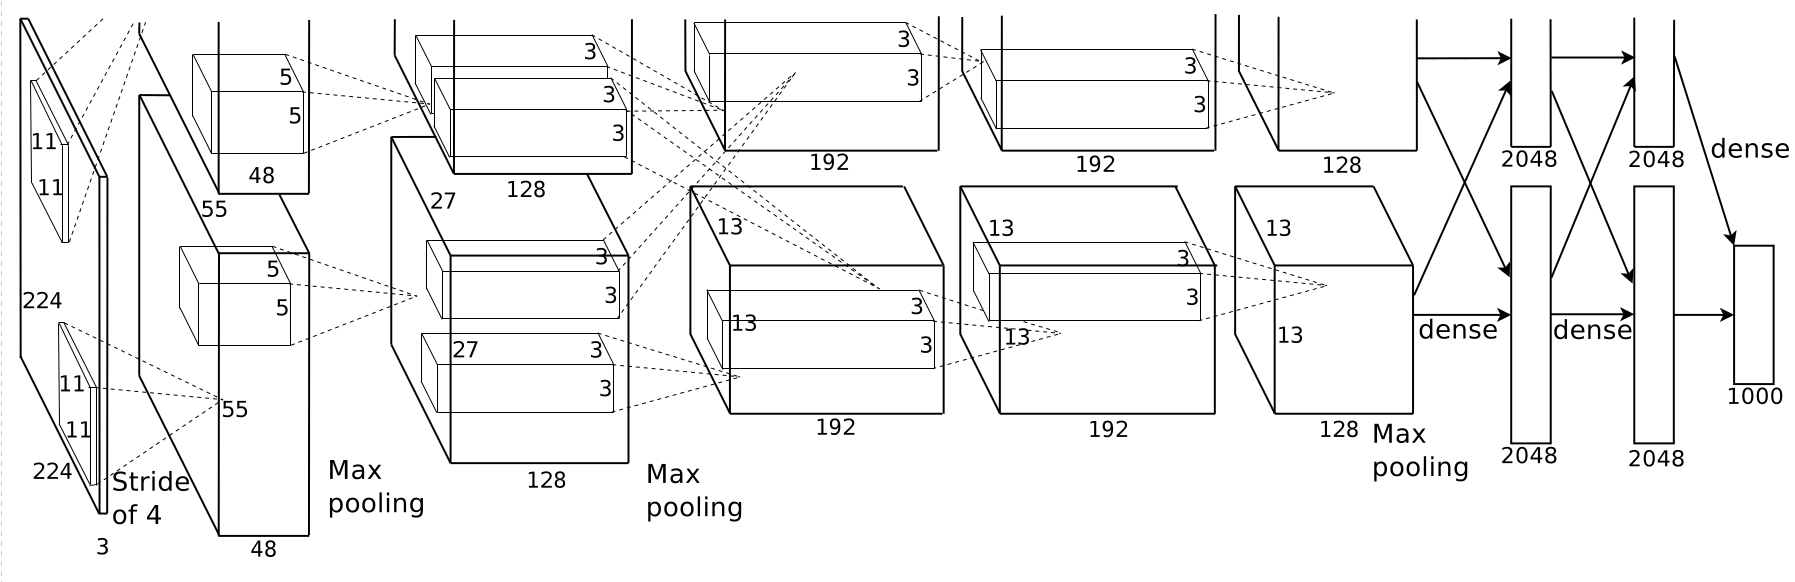
\includegraphics[width=0.98\textwidth]{cnn-architecture}
  \caption{CNN神经网络架构。\cite{krizhevsky2012imagenet}}
  \label{fig:cnn-architecture}
\end{figure}

CNN用同一个网络抽特征和分类物体类型。前面的的层是用来学
特征,然后他最后的输出层作为分类器,训练的时候统一学习整个网络模型。
虽然在CNN网络也可以把分类其与抽特征分开,用输出层前面一层作为一个4096维的Feature 
Vector,叫做CNN特征。然后可以用CNN特征同样用SVM的分类器,去掉了CNN的输出层。
\cite{Razavian_2014_CVPR_Workshops}

现在主流做法多数使用深度学习达到最先进的结果,但是SIFT特征和
特征编码与表示也还是有研究空间和应用。SIFT相关的特征计算快也
不需要一个计算量很大的学习过程。
SVM到现在一直站稳了分类器的优选位子,无论用深度学习
的特征或者SIFT都使用SVM的分类器。

\subsubsection{常用的特征与特征编码}
\label{subsubsec:image_features}
本章现在常用的特征与表示详细介绍不同特征的特点,抽取方法,缺点与亮点。
最后讲特征的转吗与表示方法的特点,转吗方法,缺点与两但。
这章把特征分成两种:人工特征与学习出来的特征。人工特征由于人手工制作的抽取
方法,基于有确定性的算法规定怎么抽取特征。学习出来的特征是基于
训练神经网络学出来特征的模型。人工特征有SIFT,SURF,HOG和其他的。
人工特点经常为特定应用场景制作,因此在某个应用能达到最先进的结果
但是无法应用在其他的应用场景。深度学习出来的特征经常可以在不同的
应用场景通用。学习出来的特征需要一个很大的数据集才能达到好的效果。
人工的特征完全不需要训练所以也不以来数据集。学习出来的特征
可以采用别人在数据集已经训练好的模型直接使用。

\paragraph{人工特征介绍}
人工特征是由于人通过有确定性的算法抽取图片的兴趣点,过滤没有用的信息。
特征的兴趣点可能是边缘,图像梯度大的地方,物体等等。
局部特征是从整个图片先找出关键点然后从关键点抽取特征描述。
全局特征是从整个图片算出特征描述,不需要找出关键点。
生下来我们介绍SIFT的局部特征,因为很多特征是积累SIFT的研究。
最后介绍一个主流的全局特征HOG。

\paragraph{SIFT特征}
SIFT(Scale-invariant feature transform,尺度不变特征转换)是
一个局部特征描述。\cite{lowe1999object}为了可靠的识别,很重要的是抽取的特征
在图像大小,旋转,噪点和声的变化中,一样可以检测到图像的兴趣点。
这样的点一般在图像的高对比度的区域,比如物体的边缘。
另外一个重要的特点是,兴趣点之间的相对位子信息不影响物体检测。
SIFT主要在物体检测和分类使用。

SIFT的算法分两段:特征关键点检测和特征描述。在特征关键点检测阶段,
SIFT找出所有兴趣点。在特征描述,SIFT从每个关键点抽取一个128维的
向量描述各个关键点。\cite{wiki:sift}
在图\ref{fig:sift-keypoints-localization}可以看到SIFT检测到的
关键点的例子,所有圈子表示一个SIFT的关键点。

\clearpage
\paragraph*{特征关键点检测}
\begin{wrapfigure}{r}{0.33\textwidth}
  \centering
    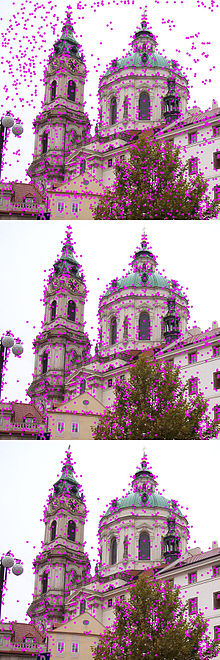
\includegraphics[width=0.32\textwidth]{sift_keypoints_localization}
    \caption{SIFT关键点检测过程。图片源:\cite{wiki:sift}}
  \label{fig:sift-keypoints-localization}
\end{wrapfigure}
SIFT特征关键点提取算法第一步,是为了边缘检测,在多个尺度用高斯滤波器,
提取不同尺度高斯模糊的图像的最大值或者最小值高斯差距。
高斯差DoG定义成$D \left( x, y, \sigma \right)$。
$D \left( x, y, \sigma \right) = L \left( x, y, k_i\sigma \right) - L \left( x, y, k_j\sigma \right)$
,这里$L \left( x, y, k\sigma \right)$是在原生的图像$I \left( x, y \right)$应用了高斯滤波器
$G \left( x, y, k\sigma \right)$,在高斯滤波器$k \sigma$表示尺度,
因此$L \left( x, y, k\sigma \right) = G \left( x, y, k\sigma \right) * I \left( x, y \right)$。
高斯差图像是尺度$k_i\sigma$高斯模糊的图像和尺度$k_j\sigma$的差距。
生产了高斯差图后,关键点是多迟到的高斯差图之间的最大值或者最小值。通过
对比,在高斯差图里的每个像素点跟8个在同一尺度像素点和9个在不同尺度的相应像素点,
算出最大值和最小值。算出来的最大或者最小值作为SIFT选择关键点。这一步,
用高斯滤波器会找出关键点叫做尺度空间极值检测。在图\ref{fig:sift-keypoints-localization}
最上面的图片,可以看到尺度空间极值检测找出的关键点。

通过尺度空间极值检测找到了太多关键点,其中有邻近太近的和不稳定的点。
所以在关键点检测第二步做关键点精确定位,丢弃低对比度的关键点和消除边缘过度的点。

首先通过二次泰勒级数展开高斯差的多尺度空间$D \left( x, y, \sigma \right)$,
做数据的内差,在不同尺度的临近关键点找出极值。
在第一步检测的候选关键点作为泰勒级数的起源。

从泰勒展开的函数取导数,从导数算出极值,然后算候选关键点到极值距离,
如果候选关键点离极值远说明有更好的候选关键点,因此可以消除本候选点。
通过求泰勒展开函数二阶导数,可以过滤掉低对比度的关键点,
如果值小于0.3可以消除候选点。

物体的边缘因为对比度高还是有很多
关键点,目标是在边缘只有几个关键点。为了达到这个效果,
SIFT算出在关键点Hessian矩阵的两个特征值,然后用两个特征值的比值过滤
消除边缘点。在图\ref{fig:sift-keypoints-localization}最下面的图片显示
边缘消除过程的效果

\paragraph*{特征关键点分配方向}
现在所有关键点有尺度不便性,但是我们也希望关键点有旋转不变性。
这一步是基于图像的梯度方向和幅度算出来。这样可以相对于方向
算出来特征描述,达到旋转不变性。
不变性算法如下:每个关键点尺度的周边的像素,使用高斯模糊的图$L \left( x, y, \sigma \right)$,
算出梯度方向和幅度。
算出梯度方向的公式:$$m \left( x, y \right) = \sqrt{\left( L \left( x+1, y \right) - L \left( x-1, y \right) \right)^2 
                  + \left( L \left( x, y+1 \right) - L \left( x, y-1 \right) \right)^2}$$
算出梯度幅度的公式:$$\theta \left( x, y \right) = \mathrm{atan2}\left(L \left( x, y+1 \right) - L \left( x, y-1 \right),
               L \left( x+1, y \right) - L \left( x-1, y \right) \right)$$
\begin{wrapfigure}{r}{0.49\textwidth}
  \centering
    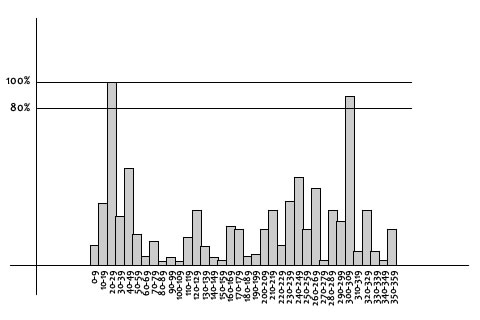
\includegraphics[width=0.48\textwidth]{sift-orientation-histogram}
    \caption{SIFT关键点梯度直方图例子。 \\
             图片源:\cite{aishack:sift-orientation}}
  \label{fig:sift-orientation-histogram}
\end{wrapfigure}
然后用一个直方图统计每个像素点的方向。直方图分成36个方块,
每一个方块表示10度,比如方块1表示所有0-9度的方向像素点,方块2表示
10-19度。那如果周边像素点方向是15度会加入到方块2,
加入的量是根据像素点幅度量添加。
做出来统计所有周边像素点梯度直方图后,可以分配关键点的主要方向和幅度。
所有直方图高峰80\%以内,创建新的在同一尺度和位子的关键点,分配相应的方向。
这个过程可以从一个关键点分成多个不同方向的关键点。
在图\ref{fig:sift-orientation-histogram}的关键点梯度方向直方图的例子,
20-29度的方块 是直方图的高峰,310-319度的方块是在高峰的80\%以内,因此本关键点
会分配20-29度的方向,同时克隆一个新的关键点分配310-319度。

\paragraph*{特征描述}
检测到了图像的关键点和分配了方向后,SIFT可以算出来每个关键点的特征描述向量,
目标是每个关键点有一个极富特色描述,但是为了后续不同图片对比还是够宽容。
SIFT描述向量,可以理解为关键点周围的局部梯度方向的直方图。

\begin{wrapfigure}{r}{0.49\textwidth}
  \centering
    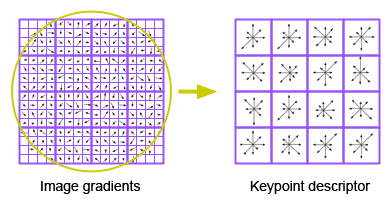
\includegraphics[width=0.48\textwidth]{sift-descriptor}
    \caption{SIFT特征描述。源:Cornell CS664}
  \label{fig:sift-descriptor}
\end{wrapfigure}
SIFT在关键点周边分出一个16x16像素区域,关键点在区域的中心,然后再
把16x16的区域分成16个4x4的区域,可以参考图\ref{fig:sift-descriptor}的
左边的图。在每个4x4的区域算出梯度方向直方图,直方图有8个方块,
每个直方图方块表示$360 / 8 = 45$度,梯度的幅度和离关键点的距离作为
直方图加入的值。因此有16个直方图,每个直方图有8个方块,最终特征描述
是所有规范化直方图的值,造成了一个$16 * 8 = 128$的向量。
在图\ref{fig:sift-descriptor}的右边可以看到描述向量的例子。


\paragraph{其他局部特征}
SIFT的成功发起了很多新的基于SIFT的特征的研究。在几年内
出了新的人工的局部特征:PCA-SIFT,SURF,FAST,BRIEF,ORB。
\cite{ke2004pca, bay2006surf, fast2006machine, calonder2010brief, rublee2011orb}
新的局部特征主要贡献点在于速度,可以更快的抽取特征,降低计算时间,因为
SIFT无法满足实时的要求。\cite{juan2009comparison, calonder2010brief}

PCA-SIFT的贡献点在于SIFT特征描述的优化,提供一个更有独特性,
更好处理图像变形和更紧凑的描述特征向量。通过实验发现PCA-SIFT
的特征描述跟其他图片特征描述对比(feature matching)运行时间
比原生的SIFT快。\cite{ke2004pca}
PCA-SIFT算法跟SIFT算法区别在特征描述的算法:SIFT使用
在关键点的周边的16x16像素点区域,PCA-SIFT用一个
41x41像素点区域。SIFT把这个区域分成8个4x4区域算出梯度直方图,
作为SIFT的128维的特征描述向量。
PCA-SIFT把41x41的区域分成用2个39x39区域,
算出横向梯度直方图和纵向梯度直方图,然后做Principal Component
Analysis降低唯独算出一个36维的特征描述响亮。
在后续研究对比了PCA-SIFT的特征发现它在描述独特性比SIFT
和其他特征差。\cite{mikolajczyk2005performance}

SURF的主要贡献点在于优化整个关键点测和特征描述的过程,做法也是被SIFT启发的。
SURF的作者说SURF运行时间快几倍,另外在不同图像变换可以更稳定检测到关键点。\cite{bay2006surf}
SIFT检测过程用多个尺度的图像算出高斯差图金字塔,在金字塔找出极值作为候选关键点。
SURF关键点检测过程,先计算积分图,然后用Hessian矩阵的行列式找出局部变化
最大的点作为候选关键点。
SURF特征描述在每个关键点,基于积分图快速计算Haar特征的总和作为
特征描述向量。

\clearpage
\begin{wrapfigure}{r}{0.49\textwidth}
  \centering
    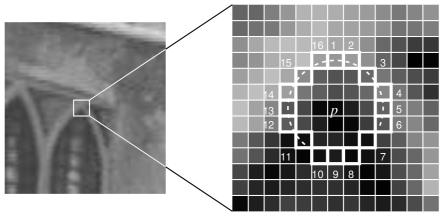
\includegraphics[width=0.48\textwidth]{fast_detector}
    \caption{FAST检测角点做法。\cite{fast2006machine}}
  \label{fig:fast-detector}
\end{wrapfigure}

FAST是一个角检测算法,没有提供描述子。
主要贡献点在于快,作者提到在实时处理视频,
SIFT和SURF都不能及时处理完视频的帧。SIFT
使用DoG(高斯差图)检测关键点,FAST提到了
一个新的方式可以检测到关键点。
FAST在每个图像像素点通过本点周边的像素点直接检查是否是一角点。
具体被检测的像素点,划分一个16个像素点的卷,然后通过16个点的不同
像素密度判断是否是角点。在图\ref{fig:fast-detector}可以看到
怎么划分16个像素点的卷。为了提高检测角点的正确率,FAST算法
用机器学习的决策树分类器。

BRIEF是一个特征描述子,没有包含关键点检测。\cite{calonder2010brief}
主要贡献点在于一个更小的用二进制表示特征描述响亮,可以
用快的Hamming距离做特征对比不同图像的BRIEF特征描述。
BRIEF描述法是在关键点取出一个模糊$S \times S$的Image Patch $p$。
BRIEF的binary test function $t$,是在Patch内的像素点对比像素密度分配boolean值:
$$
t(p; x, y) = \begin{cases} 
      1 & if p(x) < p(y) \\
      0 & else 
 \end{cases}
$$
这里$p(x)$是像素点$x$在模糊的patch $p$的像素密度。选择$n_d$个$(x, y)$
对作为BRIEF的$n_d$长度的特征描述。作者推荐$n_d$使用128, 256, 512,太小了
会影响特征描述的独特性,但是太大了对存储和计算需求有影响。

ORB是一个基于FAST角点检测器和BRIEF特征描述子的特征,
重点是提供一个效果跟SIFT一样但是可以实时计算的特征。
主要贡献是提供旋转不变性和提高图像噪点抵抗性,原生的
FAST和BRIEF都却的。ORB推出了oFAST(Orientated FAST),
先创建一个多尺度的图像金字塔,在每个金字塔的level用FAST
检测关键点然后,按Harris的corner measure顺序选前$n$个关键点。
通过多尺度金字塔可以提供尺度不变性。在每个检测到关键点
ORB使用Intensity Centroid算出方向。
另外ORB推出了rBRIEF特征描述,是一个旋转不变的BRIEF。ORB
先旋转image patch然后再算出BRIEF特征描述。作者通过实验发现
旋转的BRIEF特征描述的反差比原生BRIEF大,影响特征描述的独特性。
通过一个自己的算法ORB学习怎么更好的选无相关的$(x, y)$对做
binary test,这样降低旋转BRIEF的方差。


\paragraph{全局特征 - HoG}
全局特征从整个图像算出特征描述,不需要一个特征关键点检测的过程。
在2005年,N. Dalal和B. Triggs推出了HoG(Histogram of Gradients)
方向梯度直方图。\cite{dalal2005histograms}
当时用在图像的人类识别,检测图像哪里有人类。另外的应用场景包括
物体识别,场景识别和视频里的人类识别。HoG也是收一个被SIFT
启发的特征。

\begin{wrapfigure}{r}{0.49\textwidth}
  \centering
    \captionsetup{justification=centering}
    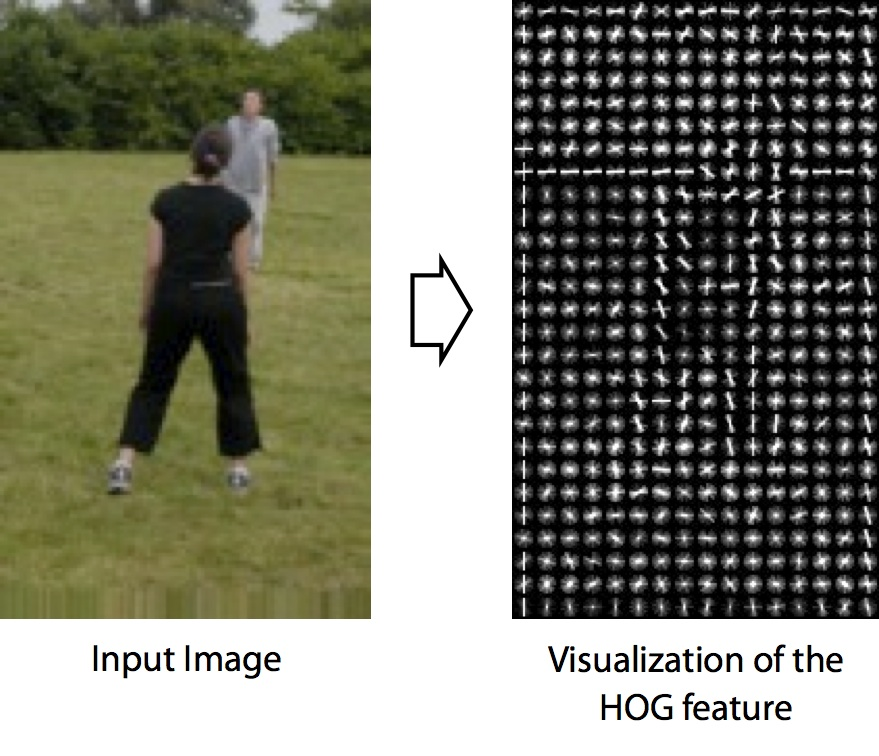
\includegraphics[width=0.48\textwidth]{hog-visualization}
    \caption{可视化HOG的特征描述。\\
             源:Cornell CS4670}
  \label{fig:hog-visualization}
\end{wrapfigure}
HoG的算法把整个图像分成$n$个连在一起的区域(cells),每个区域先单独算出来
它的梯度方向与梯度直方图。为了考虑照明和对比度的变化,HoG把多个区域
连在一起然后归一化。所有区域归一化后的直方图作为HoG的特征描述响亮。
在图\ref{fig:hog-visualization}可以看到图像到HoG特征的可视化。

在论文里面用了SVM分类器,用HoG的特征描述向量输入到SVM。
作者在MIT pedestrian database训练了和测试了HoG + SVM的
人类识别性能,几乎能正确识别整个测试数据集。因此作者
再做了一个新的更有挑战和大的人类识别数据集。


\paragraph{深度学习特征}
深度学习特征用机器学习的算法自动学出来图像的特征抽取与表示方法。
在人脸识别,物体识别还有其他场景,学习出来的特征获得了现在先进的结果。
\cite{taigman2014deepface, krizhevsky2012imagenet}
在2014年,Razavian研究了用CNN作为特征在其他应用场景,对比CNN和基于SIFT
的效果。在它测试数据集和应用场景,基于CNN的特征的效果,都比基于人工特征的方法好。
\cite{razavian2014cnn}

%Deep Learning Features, mainly explain CNN and how we can use it as feature.
%R-CNN, SPP, Fast R-CNN, Faster R-CNN, CDBN(Convolutional Deep Belief Network)

%Edge Detection
%DeepEdge, DeepCountour


\subsubsection{特征转吗与图像表示}
在图\ref{fig:image-representation}可以看到经典的工作流。
第一步从图片抽取特征描述比如SIFT,
第二部从特征描述转吗到图像表示(Image Representation),
然后图像表示用于在分类器的训练和分类。
特征转吗用一个词典(Visual Codebook)分配每个特征描述行属于
哪个词,总结这个信息作出一个图像表示响亮。
使用特征编码与图像表示,可以帮助提高识别类型的通用性。比如需要分类器
在鉴于,影像,灯光和闭塞变化中,还是能识别出属于同一个类型。
最早的方法是在2004年发布的Visual Categorization with Bag of Keypoints,
应用了Bag-of-Words的模型在机器视觉的任务。\cite{csurka2004visual}
后续基于BoW改进的方式包含 Fisher Vector转吗和VLAD。
\cite{perronnin2007fisher,jegou2010vlad}本章先介绍BoW理解转吗和词典生产的过程,
然后介绍Fisher Vector和VLAD怎么改进BoW。
\begin{figure}
  \centering
    \includegraphics[width=0.98\textwidth]{image-representation}
    \caption{特征转吗到图像表示的过程。}
  \label{fig:image-representation}
\end{figure}

Bow Intro, Dictionary Generation, Encoding, Classifier example

\subsubsection{常用的分类器}
\label{subsubsec:classifier}
Based on probability, SVM, Naive Bayes

\subsubsection{数据集}

MNIST, Caltech, VOC, ImageNet

\subsubsection{相关的软件}
OpenCV, Caffe, vlfeat, scikit


\subsubsection{结论}
Relationship of background to CloudVision

\subsection{大数据与分布数处理研究现状}
\label{subsec:bigdata_background}
数据增长从稀缺到过多,带来新的好处,但是同时也带来新的挑战。
互联网公司一直跟数据的快速曾长在战斗。谷歌(Google)每天处理24PB的数据。
Facebook的用户每小时保存1000万个图片,每天用户点赞30亿次。点赞的数据
可以用来分析用户的兴趣和爱好,推出更有效的广告。
除了互联网公司之外,其他行业也面对数据成倍曾长的情况,同样想抓我新的机会。
沃尔玛公司(Wal-Mart Stores Inc.),来自与美国是一个在全球运营超市连锁企业,
每小时处理100万的交易,保存到一个超过2.5PB的数据库,从这些数据沃尔玛找出买家的模式。
数据在各个行业变了一个很重要的无形资产。\cite{mayer2013bigdata}

大数据领域属于所有数据超过传统存储容量和处理能力,利用这些海量数据
得到商务的优势。可以用3V数据曾长模型描述数据:
\begin{itemize}
  \item Volume(数据量): 数据的大小比如1PB。
  \item Velocity(速):数据的输入和输出速度,比如每分钟保存1TB新数据。
  \item Variety(多样性):数据包含不同的数据类型,比如文本,视频,图像,社交网络等等。
\end{itemize}
Gartner用3V模型定义成大数据:"大数据是量特别大,高速曾长,多样性的数据
,这些数据为了创造价值需要特殊的技术与分析模型。"\cite{bigdatadefinition}

在2004年Google发布了"MapReduce:简单化集群的数据处理",描述Google内部用的
模型和技术解决大数据的挑战。\cite{dean2008mapreduce}
MapReduce是一个框架,用来在集群并行处理大数据。MapReduce程序组成一个Map(映射)函数和
Reduce(归纳)函数。Map函数一般用来过滤和数据预处理,然后由Reduce函数总结数据比如算出平均值。
用MapReduce函数是一个从函数变成范式借过来的。MapReduce贡献点是在于提出怎么在集群里高效与可靠
并行执行MapReduce程序。MapReduce使用数据的局部性,处理数据在接近的节点减少数据移动。

在2006年Doug Cutting被Google FileSystem和MapReduce收到启发开发了开源的Apache Hadoop。
\cite{gfs2003, dean2008mapreduce, wiki:hadoop}Apache Hadoop是一个开源框架提供
,在普通硬件上的大数据集分布式存储与处理。Hadoop变了一个世界上的大数据技术标准,
大互联网公司和企业都在用,典型的包含Facebook,Baidu,Yahoo,Ebay,Spotify。
在本章\ref{subsubsec:hadoop}会详细介绍Hadoop的框架和架构。

在2009年,UC Berkeley的AMPLab开始开发了Spark,一个开源集群分布式处理框架。\cite{wiki:spark}
Spark改善了MapReduce分布式框架,用内存运算技术提高性能,另外提供一个更灵活
的编程范式,不限于用Map/Reduce函数。Spark编程范式,合适于机器学习的算法和其他
迭代形式的算法。在本章\ref{subsubsec:spark}会详细介绍Spark。



\subsubsection{Apache Hadoop}
\label{subsubsec:hadoop}
Apache Hadoop是一个开源被Apache维护的分布式存储与处理框架。
Hadoop所有模块都设计到,如果任意件硬件所发生故障不影响数据丢失
和处理的结果。
Apache Hadoop框架核心模块有:
\begin{itemize}
  \item Hadoop Common:所有模块用的程序库和工具。
  \item Hadoop Distributed File System(HDFS):分布式存储文件系统,使用普通的电脑与服务器提供
        高效,容量大的可靠的存储集群。
  \item Hadoop MapReduce:一个基于Google提出的MapReduce范式分布式处理实现集群分布式处理。
  \item Hadoop YARN:集群资源管理,用来调度用户提交的分布式处理任务,比如调度MapReduce任务。
\end{itemize}
除了Apache Hadoop核心之外,Hadoop也变成了一个生态系统,HBase(基于HDFS的NoSQL),Hive(数据仓库)等等都属于
Hadoop的生态系统。Apache Hadoop大部分代码用Java写的,少部分脚本用Python写的,还有少部分Native代码用C写的。

\paragraph*{Hadoop Distributed File System}
HDFS是Hadoop实现的分布式,可扩展,高可用文件系统。一个HDFS集群分两种主要节点:Namenode和Datanode。
HDFS集群一般有一个Namenode,由它保存记录和目录的层次和namespace(命名空间)。Namenode使用inodes表示文件和目录。Inode记录
文件和目录的属性比如权限,修改与访问时间,空间配额和命名空间。HDFS把文件的内容分成多个blocks(块),默认一块是128MB,
然后将每个块独立复制到多个(默认是3个)不同的datanodes。Namenode维护一个命名空间对应块的树,记录文件所有块保存在
那个datanode。

在图\ref{fig:hdfs-arch}描述HDFS的集群架构,为简单起见当时集群保存了一个350MB的文件,名字是example.txt。
文件会分成$\ceil{\frac{350}{128}} = 3$个块,分别为B1,B2,B3。每一块需要保存3份到不同的datanode。

\begin{figure}
  \centering
    \includegraphics[width=0.85\textwidth]{hdfs-arch}
    \caption{HDFS的集群架构。}
  \label{fig:hdfs-arch}
\end{figure}


\paragraph*{Hadoop Compatible File System}

\paragraph*{Hadoop Map/Reduce}


\subsubsection{Apache Spark}
\label{subsubsec:spark}
Spark History, Arch, HA

\subsubsection{Apache Mesos}


\subsubsection{大数据总结}

\subsection{云计算领域研究现状}
\label{subsec:cloud_background}
云计算是通过网络按需求提供计算资源(比如服务器,网络,存储,应用,服务),资源可以快速调配和解放,
调配与解放需要运营商的没有或者少量管理工作。

\subsubsection{Amazon AWS}
S3 and compute

\subsubsection{OpenStack}
\label{subsubsec:openstack}
Swift and compute

\subsection{自动部署现况}
\label{subsec:automated_deployment}

Introduce Ansible, Roles, Playbooks. Refer to Chapter

\subsection{基于大数据实现大规模机器视觉的研究现况}
\label{subsec:bigdata_cv_background}

\section{问题与挑战}
\label{sec:challenges}

\section{本文主要工作在与结构安排}
\label{sec:main_work}

Research on latest state-of-the art, architecture

Development of all components: REST-API, UI, Spark algorithms,

OpenStack Private Cloud Deployment


\chapter{CloudVision架构与设计}
\label{cha:architecture}
在图\ref{fig:cloudvision-arch}可以看到CloudVision的架构主要分成两部分:
控制与管理层和业务与处理层。用户可以通过Web UI,CLI或者API使用
CloudVision的服务。 控制层提供对外的服务然后业务层负责在大数据平台
处理任务。控制与管理层和业务与处理层之间
基于一个消息队列转达任务和信息。通过分开控制层和处理层我们可以
独立扩展两部分,也保持它们独立性。如果处理性能不足可以
增加处理层的服务器。
\begin{wrapfigure}{r}{0.5\textwidth}
  \centering
  \includegraphics[width=0.48\textwidth]{cloudvision-arch}
  \caption{CloudVision 总体架构}
  \label{fig:cloudvision-arch}
\end{wrapfigure}
控制与管理层负责:
\begin{itemize}
  \item 对外提供\textbf{API}: 通过HTTP提供一个完整的RESTFUL API;
  \item 管理\textbf{云平台}: 在OpenStack或者亚马逊的AWS创建基础设施的资源;
  \item 管理\textbf{大数据处理集群}: 自动部署和搭建大数据集群在云平台上面;
  \item 管理机器视觉的\textbf{任务}: 添加用户自己写的或者执行CloudVision自带机器视觉的任务。
  \item 管理不同的\textbf{数据源}: 管理对象存储的数据源作为机器视觉任务的输入和输出。
\end{itemize}
业务与处理层主要负责执行机器视觉相关的任务:
\begin{itemize}
  \item \textbf{特征抽取}: 提供主流的特征比如CNN,SIFT和SURF。
        用户也可以自己添加新的特征抽取算法;
  \item \textbf{机器学习}: 提供基础的机器学习和分类器。
        比如K-Means,Deep Neural Networks和SVM。
  \item \textbf{抽帧}: 从多个视频抽帧然后保存到数据源或者
        分布式内存存储;
  \item \textbf{内存缓存}: 提供高效零时的存储;
\end{itemize}

在本章接下来的章节会详细介绍架构里面的每一部分。最终通过实验的方式
证明横向扩展性和不用架构的架构优势。


\section{控制与管理层}
\label{sec:arch_control}
在图\ref{fig:cloudvision-arch-control}可以看到CloudVision的
控制与管理层内部的架构。客户段通过API层提供的HTTP REST API使用
CloudVision的服务。然后CloudVision保存所有持久数据到MongoDB的数据库。
API层通过AMQP协议发信息到信息队列。然后由API workers从
信息队列收到的任务后,启动长期的业务处理的任务比如
创建虚拟机,部署集群,在集群执行机器视觉任务等等。

\begin{figure}[h]
  \centering
    \includegraphics[width=0.85\textwidth]{cloudvision-arch-control}
  \caption{CloudVision 控制与管理层架构和实现}
  \label{fig:cloudvision-arch-control}
\end{figure}

\subsection{客户端}
CloudVision提供两种不同的客户段:Web界面和Python REST Client/CLI。
Web客户段是为了让用户容易使用CloudVision的平台,不需要让用户了解细节的API接口。
Web段是基于Angular2和HTML Bootstrap框架开发,Web所有逻辑全部在浏览器运行。
由Agular2从用户的浏览器直接通过AJAX HTTP请求调用CloudVision服务器段的REST API。

\subsection{API层}
API层是跑在CloudVision的服务器段提供对外的服务。它负责
收到HTTP请求,保存数据然后把任务转到信息队列,转完了回HTTP应答。
CloudVision的RESTP API定义五种资源:Cloud(基础施舍云),Cluster(处理集群),
Job(任务),Job Template(任务模板),Datasource(数据源)。

\begin{table}[htb]
  \centering
  \begin{minipage}[t]{0.95\linewidth} % 如果想在表格中使用脚注,minipage是个不错的办法
  \caption[CloudVision API接口列表]{CloudVision API接口列表。}
  \label{tab:template-files}
    \begin{tabularx}{\linewidth}{lXlXlXlXl}
      \toprule[1.5pt]
        资源URI & GET & PUT & POST & DELETE \\
        \$base/clouds & 返回用户所有云平台。支持分页,默认提供10件。 & 没使用 & 添加用户的基础施舍云API访问信息 & None \\
        \$base/clouds/\{uuid\} & 返回所有云平台 & None &  None & None \\

      \bottomrule[1.5pt]
    \end{tabularx}
  \end{minipage}
\end{table}



\subsection{基础设施云管理}
\subsection{大数据与处理集群管理}
\subsection{机器视觉任务管理}
\subsection{数据源管理}


\section{业务与处理层}
\label{sec:arch_workers}

\section{基础设施层}
\label{sec:arch_infra}


\section{架构对比和实验}
\label{sec:arch_experiment}

\chapter{分布式机器视觉库}
\label{cha:distributed_vision_library}
Describe existing re-usable implementations

\section{媒体存储结构}
在大数据存储比如HDFS和对象存储高效批量处理小文件是一个问题。
这里定义小文见是文件大小小于大数据存储的block size。Hadoop
HDFS默认定义的block size是64MB。Swift和S3对象存储默认
block size是32MB。图片大小一般是10KB - 200KB。
如果直接保存图片,每个图片是一个独立的文件会
造成处理的时候得每个图片单独读取,发多个请求。
另外处理的时候Spark和Hadoop Map/Reduce也
无法同时处理多个图片在同一个任务。

目前在CloudVision通过两个方式解决高性能
批量处理小文件的问题:使用SequenceFiles和
Apache Parquet的存储格式和方式。SequenceFile提供
图片存储,Parquet提供中间结果存储结构。


\subsection{基于SequenceFile存储大量图片}
Hadoop的SequenceFile格式可以保存Key/Value对。
CloudVision使用SequenceFile保存大量的图片,Key是一个
string用来保存图片文件名字,Value是一个Array[Bytes]用来保存
图片的内容。

SequenceFile可以被分段(splittable),这样Spark或者Map/Reduce的任务
可以同时分别处理不同的分段,提高处理性能和并行化。

\begin{figure}[h]
  \centering
    \includegraphics[width=0.98\textwidth,trim=1 1 4 1,clip]{cloudvision-seqfile}
  \caption{CloudVision 保存图片的SequenceFile格式和用法}
  \label{fig:cloudvision-seqfile}
\end{figure}

在图\ref{fig:cloudvision-seqfile}有一个例子保存整个ImageNet2015数据集。
黄色表示Key保存文件名字:1.jpg和蓝色表示图片的裸的bytes。SequenceFile可以有
$N$个条目。

为了容易让用户转换和上传数据集,CloudVision自开发了一个工具。
在Listing \ref{lst:uploadseqfile}提供了几行工具主要代码。
工具的输入是一个图片目录和输出目录,它从图片目录读取所有
文件文件名和内容,创建出来一个SequenceFile在输出目录,
将每个图片文件保存到SequenceFile里。比如用户可以这样
调用工具:
upload\_to\_seqfile /home/sam/imagenet2014 swift://spark.swift/imagenet2014.hseq,
会将用户本地/home/sam/imagenet2014图片目录上传到Swift的对象存储保存一个SequenceFile,
Swift里面文件名是imagenet2014.hseq。

\begin{lstlisting}[language=Java,
                   basicstyle=\tiny,
                   showstringspaces=false,
                   caption={UploadToSequenceFile工具},
                   label={lst:uploadseqfile}]
Path outputPath = new Path(outputPath);
writer = SequenceFile.createWriter(conf, SequenceFile.Writer.file(seqFilePath), 
            SequenceFile.Writer.keyClass(Text.class),
            SequenceFile.Writer.valueClass(BytesWritable.class));
for (File file : imageFiles) {
    byte buffer[] = Files.toByteArray(file);
    writer.append(new Text(file.getName()), new BytesWritable(buffer));
}
writer.close();
\end{lstlisting}

在后续的Spark任务可以通过SparkContext.sequenceFile直接读取SequenceFile。
Spark会自动把Key,Value Pairs做成一个RDD。在章\ref{sec:feature-extraction}
会有详细的例子使用图片的SequenceFile抽取特征。

\subsection{基于Parquet通用数据结构}
Parquet是提供一个通用的数据列式存储。列式存储
按列保存数据,特别合适在批量处理使用。CloudVision
主要用Parquet来保存所有处理的结果,比如从图片抽取的
特征或者图像表示。
在CloudVision选上了Parquet的原因有:
\begin{itemize}
  \item 通用性 \\
        不同的处理平台都
        支持Parquet的格式包含Spark, Hadoop Map/Reduce和Cascading。
  \item 高效I/O \\
        因为度数据的时候不需要扫描。Parquet列式存储底层使用blocks保存,
        可以按整个block做一次IO请求读取block里面所有数据。另外可以
        只选需要读取的列,降低需要读取的大小。
  \item 高效压缩 \\
        Parquet的压缩编码能减少存储使用的大小。
  \item Spark SQL的DataFrame兼容性 \\
        Spark natively支持Parquet的格式。通过Spark SQL可以直接
        读取Parquet文件转成DataFrame,同样DataFrame可以直接
        写成Parquet文件。
\end{itemize}



\section{特征抽取}
\label{sec:feature-extraction}
Hand-crafted features SIFT, SURF, HOG,
First one to publish and succeed extracting SIFT/SURf features on Spark efficiently
Learned Features CNN


\section{特征编码与表示}
Classic BoW with sparse vecotrs
VLAD with distances and pooling same codebook as BoW
Feature Detection -> Feature Descriptors -> Codebook Generation
Feature Descriptors -> Codebook assign -> BoW -> Pooling -> 


\section{机器学习与分类器}
SVM, 

\chapter{CloudVision - 机器视觉云平台}
\label{cha:cloudvision_cloudplatform}

placeholder


\chapter{结论和未来工作}

Show screenshots of Github stars. Plan to add more support for deep learning algorithms including tensorflow.

Future work:
More Deep Learning support (TensorFlow, CaffeOnSpark, deeplearning4j, SparkNet)
Object Detect API on top of PaaS



%%% 其它部分
\backmatter

%% 本科生要这几个索引,研究生不要。选择性留下。
% 插图索引
\listoffigures
% 表格索引
\listoftables
% 公式索引
\listofequations


%% 参考文献
% 注意:至少需要引用一篇参考文献,否则下面两行可能引起编译错误。
% 如果不需要参考文献,请将下面两行删除或注释掉。
\bibliographystyle{thuthesis}
\bibliography{ref/refs}


%% 致谢
% 如果使用声明扫描页,将可选参数指定为扫描后的 PDF 文件名,例如:
% \begin{ack}[scan-statement.pdf]
\begin{acknowledgement}
  衷心感谢导师丁贵广副教授对本人的精心指导。他推荐的题目特别合适我的兴趣,让我更有动力
  和自由的作出好结果。他的言传身教将使我终生受益。

  另外感谢,我老婆,也是学姐,林丹,不停的鼓励和支持我,还帮忙复习和修改语法和错字。
  在没有她帮忙下,估计其他人就很难看懂我的论文。

  感谢ThuThesis的LaTeX模板,它的存在让我的论文写作轻松自在了许多,让我的论文格式规整漂亮了
  许多。
\end{acknowledgement}


%% 附录
%\begin{appendix}
%\input{data/appendix01}
%\end{appendix}

%% 个人简历
%\begin{resume}

  \resumeitem{个人简历}

  1990 年 05 月 05 日出生于 在荷兰的Delft城市。

  2007 年 09 月考入 The Hague University 的 ICT 系 Informatica 专业,2011 年 07 月本科毕业并获得 Bachelor of ICT in Informatica  学士学位。

  2011 年 08 月 至 2012 年 06 月,自由职业Web后台开发者

  2012 年 06 月 至 2013 年 08 月,在一家云计算公司做OpenStack的研发,也给OpenStack开源社区贡献代码。

  2013 年 09 月免试进入清华大学软件学院攻读软件工程学位至今。

\end{resume}

\end{document}
